% Provenance (never printed): see sources/outline_sources.md and sources/book1/BRIEFS.md (g6/01).
\chapter{A First Python Program}\label{ch:g6:first-python-program}

Sami's family is going shopping, and the list is long, with a price next
to each item. Sami starts adding them up with a pencil. His sister types one line on
the laptop and presses \key{Enter}: the total appears before Sami has added the
first three prices. She did not use a calculator. She wrote a tiny \omterm{def:g4:programs-and-operating-system:program}{program}. From
this chapter on, we write \omterm{def:g4:programs-and-operating-system:program}{programs} ourselves, in a language called Python.

\begin{recall}
A \omterm{def:g4:programs-and-operating-system:program}{program} is a list of \omterm{def:g1:instructions-in-order:instruction}{instructions} for a \omterm{def:g1:what-is-a-computer:computer}{computer}, kept as a \omterm{def:g3:files-and-folders:file}{file}
(\cref{ch:g4:programs-and-operating-system}); \omterm{def:g1:instructions-in-order:instruction}{instructions} are carried out one
after another, in order (\cref{ch:g1:instructions-in-order}); an \omterm{def:g4:algorithms-repeat-and-decide:algorithm}{algorithm} is a
precise method that always ends (\cref{ch:g4:algorithms-repeat-and-decide}).
\end{recall}

\section{A language precise enough for a machine}

People understand a sentence even when it is not quite right. A \omterm{def:g1:what-is-a-computer:computer}{computer}
cannot guess: it needs \omterm{def:g1:instructions-in-order:instruction}{instructions} written with a few words and strict rules.

\begin{definition}[Programming language]\label{def:g6:first-python-program:language}
A \emph{programming language}\index{programming language} is a language for
writing \omterm{def:g4:programs-and-operating-system:program}{programs}: a small set of words and signs, with strict rules saying
what each one means, so that the \omterm{def:g1:what-is-a-computer:computer}{computer} can carry out the \omterm{def:g4:programs-and-operating-system:program}{program} exactly.
\end{definition}

There are hundreds of \omterm{def:g6:first-python-program:language}{programming languages}. This book uses Python, which is
easy to read and used all over the world, by beginners and by experts. A
Python \omterm{def:g4:programs-and-operating-system:program}{program} gives the same result on every \omterm{def:g1:what-is-a-computer:computer}{computer} that runs it.

\begin{history}[A language named after a comedy show]
% ledger: g6:python-origin, g6:python-name
Python was begun by Guido van Rossum during the Christmas holidays of 1989 and
first shared with other programmers in February 1991. He was reading the
scripts of a British comedy series of the 1970s, \emph{Monty Python's Flying
Circus}, and wanted a name that was short and a little mysterious.
\end{history}

\section{The editor and the interpreter}

\begin{definition}[Source file]\label{def:g6:first-python-program:source}
A \emph{source file}\index{source file} is the text \omterm{def:g3:files-and-folders:file}{file} in which a \omterm{def:g4:programs-and-operating-system:program}{program}
is written. Python source \omterm{def:g3:files-and-folders:file}{files} end with the \omterm{def:g3:files-and-folders:extension}{extension} \code{.py}.
\end{definition}

A \omterm{def:g6:first-python-program:source}{source file} is written in a \omterm{def:g2:using-a-computer:word-processor}{text editor}, like any other text. To run it, we
give it to another \omterm{def:g4:programs-and-operating-system:program}{program}.

\begin{definition}[Interpreter]\label{def:g6:first-python-program:interpreter}
The Python \emph{interpreter}\index{interpreter} is the \omterm{def:g4:programs-and-operating-system:program}{program} that reads a
Python \omterm{def:g6:first-python-program:source}{source file} and carries out its \omterm{def:g1:instructions-in-order:instruction}{instructions}, one after another.
\end{definition}

\begin{omfigure}
\begin{tikzpicture}[x=1cm, y=1cm, font=\footnotesize]
  \omwindow{3.6}{2.4}{hello.py}
  \pic at (0,0) {window};
  \foreach \y/\w in {1.55/2.9, 1.15/3.1} \draw[ocBlue!70, line width=2pt] (0.3,\y) -- (\w,\y);
  \node[draw=black!70, fill=ocYellow!35, rounded corners=3pt, minimum width=2.6cm, minimum height=1.2cm, align=center] (int) at (6.0,1.2) {Python\\interpreter};
  \draw[black!80, fill=black!85, rounded corners=2pt] (8.4,0) rectangle (12.2,2.4);
  \node[anchor=west, text=white, font=\scriptsize\ttfamily, align=left] at (8.55,1.2) {Hello! I am a program.\\I run the same way\dots};
  \draw[-{Stealth[length=2.5mm]}, thick] (3.7,1.2) -- node[above] {reads} (int.west);
  \draw[-{Stealth[length=2.5mm]}, thick] (int.east) -- node[above] {prints} (8.35,1.2);
  \node[font=\footnotesize] at (1.8,-0.35) {source file};
  \node[font=\footnotesize] at (10.3,-0.35) {terminal: the output};
\end{tikzpicture}

{\small The \omterm{def:g6:first-python-program:interpreter}{interpreter} reads the \omterm{def:g6:first-python-program:source}{source file} and carries out its \omterm{def:g1:instructions-in-order:instruction}{instructions};
what the \omterm{def:g4:programs-and-operating-system:program}{program} prints appears in a terminal window.}
\label{fig:g6:first-python-program:interpreter}
\end{omfigure}

Here is our first \omterm{def:g4:programs-and-operating-system:program}{program}. Every \omterm{def:g4:programs-and-operating-system:program}{program} in this book is printed like this,
with its line numbers on the left and its \omterm{def:g3:files-and-folders:file}{file name} under it.

\Needspace*{5\baselineskip}
\omcode{code/grade-6/01-first-python-program/listings/hello.py}{1}{2}{Two
greetings.}\label{lst:g6:first-python-program:hello}

To run it, we type a command in a terminal: the word \code{python}, then the
name of the \omterm{def:g3:files-and-folders:file}{file}. Every \omterm{def:g1:what-is-a-computer:input}{output} in this book starts with that command, after a
\texttt{\$} sign, then shows what the \omterm{def:g4:programs-and-operating-system:program}{program} printed.

\Needspace*{6\baselineskip}
\omoutput{code/grade-6/01-first-python-program/outputs/hello.txt}{The command
that runs the \omterm{def:g4:programs-and-operating-system:program}{program}, then its two lines.}\label{out:g6:first-python-program:hello}

Python can also be used without a \omterm{def:g3:files-and-folders:file}{file}: typing \code{python} alone opens an
\emph{interactive prompt}, where each line is run as soon as \key{Enter} is
pressed. It is handy for trying a calculation; for \omterm{def:g4:programs-and-operating-system:program}{programs}, we always use
\omterm{def:g3:files-and-folders:file}{files}, so that they can be saved, corrected and run again.

\begin{omfigure}
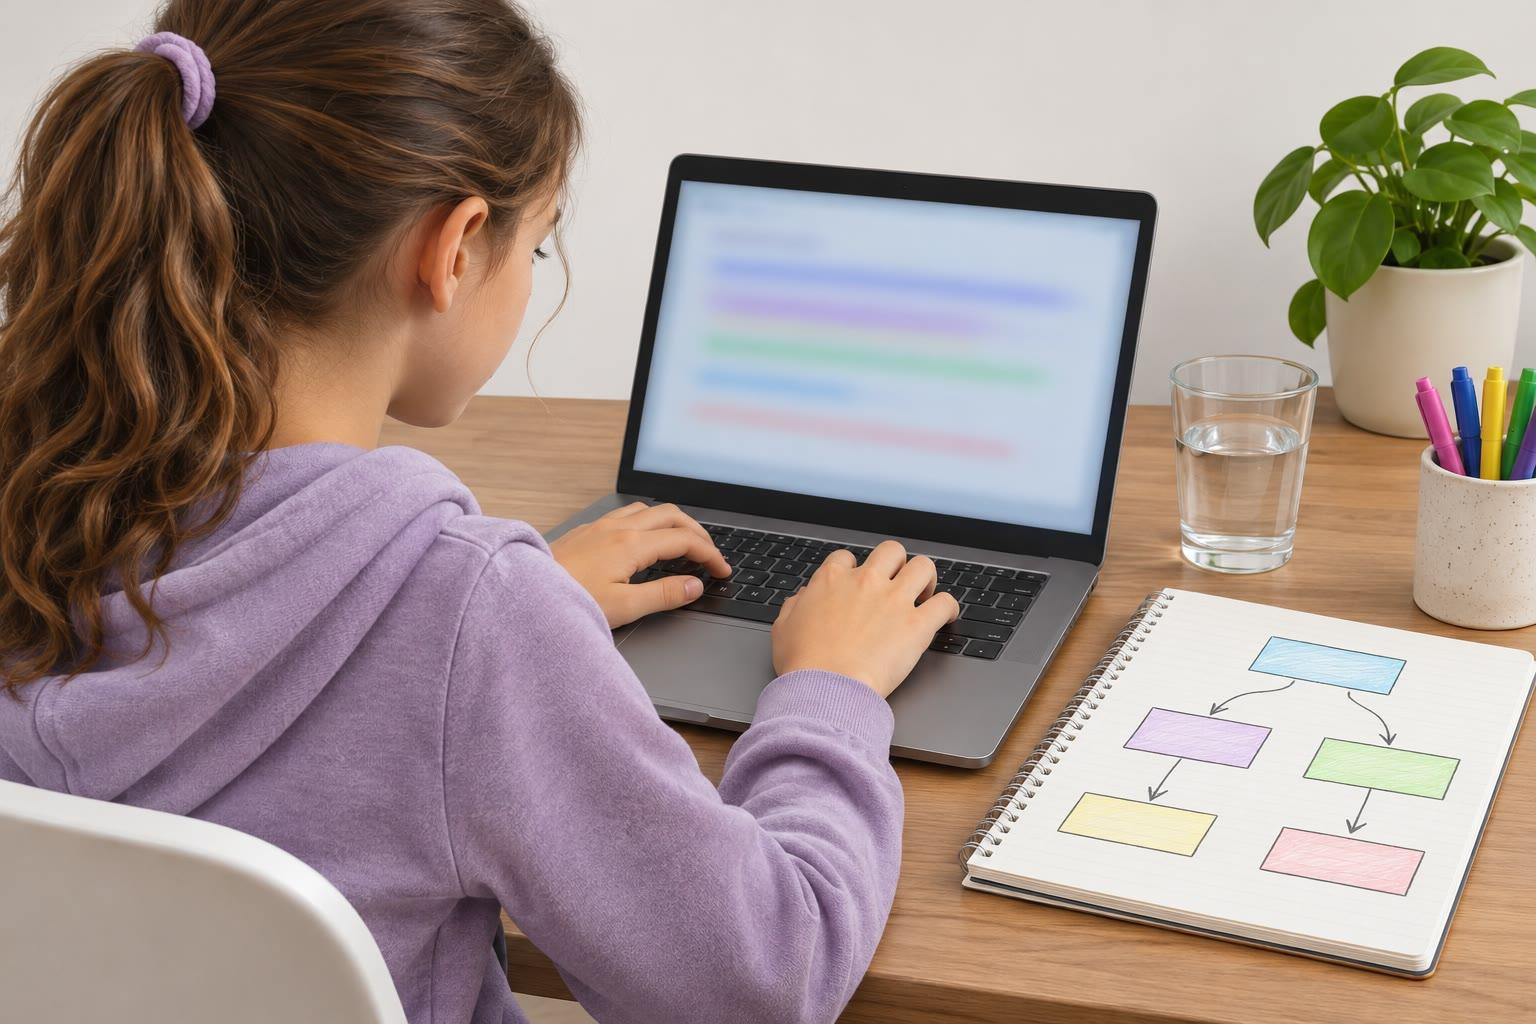
\includegraphics[width=0.48\linewidth]{images/book1/ai/g6-first-python-program-desk.jpg}

{\small Writing a first \omterm{def:g4:programs-and-operating-system:program}{program}, with the plan drawn on paper beside the
laptop.}
\end{omfigure}

\section{\texorpdfstring{\code{print}}{print} and numbers}

The \omterm{def:g1:instructions-in-order:instruction}{instruction} \code{print} shows on the screen what is between its brackets.
Text is written between double quotes; a calculation is written without quotes,
and \code{print} shows its result. This is how Sami's sister added up the
prices:

\Needspace*{5\baselineskip}
\omcode{code/grade-6/01-first-python-program/listings/prices.py}{1}{2}{Adding
up a shopping list.}\label{lst:g6:first-python-program:prices}

\Needspace*{5\baselineskip}
\omoutput{code/grade-6/01-first-python-program/outputs/prices.txt}{The total, in
euros.}\label{out:g6:first-python-program:prices}

The first line starts with \texttt{\#}: it is a sentence for people, which Python
skips (more about this below). Python knows the four operations of arithmetic,
written \code{+}, \code{-}, \code{*} (times) and \code{/} (divided by). The
point, not a comma, separates the whole part of a number from its decimals.

\Needspace*{8\baselineskip}
\omcode{code/grade-6/01-first-python-program/listings/operations.py}{1}{5}{The
four operations.}\label{lst:g6:first-python-program:operations}

\Needspace*{9\baselineskip}
\omoutput{code/grade-6/01-first-python-program/outputs/operations.txt}{A division
always gives a decimal number, even when it falls
exactly.}\label{out:g6:first-python-program:operations}

Look at the last line: $10 / 2$ prints \code{5.0}, not \code{5}. The sign
\code{/} always gives a decimal number. For sharing things that cannot be cut,
Python has two more operations: \code{//} gives the whole number of times
(the quotient of the division with a remainder), and \texttt{\%} gives what is
left over (the remainder).

\Needspace*{6\baselineskip}
\omcode{code/grade-6/01-first-python-program/listings/share.py}{1}{3}{Sharing 23
sweets between 5 friends.}\label{lst:g6:first-python-program:share}

\Needspace*{6\baselineskip}
\omoutput{code/grade-6/01-first-python-program/outputs/share.txt}{4 sweets each,
and 3 left over.}\label{out:g6:first-python-program:share}

\begin{omfigure}
\begin{tikzpicture}[x=1cm, y=1cm, font=\footnotesize]
  \foreach \g in {0,...,3} {
    \draw[black!50, rounded corners=4pt, fill=ocBlue!8] (2.3*\g,0) rectangle ++(2.0,1.2);
    \foreach \k in {0,...,4} \fill[ocRed!75!black] ({2.3*\g+0.3+0.35*\k},0.6) circle (0.13);
    \node at (2.3*\g+1.0,-0.3) {friend \the\numexpr\g+1\relax};
  }
  \draw[black!50, rounded corners=4pt, fill=ocBlue!8] (9.2,0) rectangle ++(2.0,1.2);
  \node at (10.2,-0.3) {friend 5};
  \foreach \k in {0,...,4} \fill[ocRed!75!black] ({9.5+0.35*\k},0.6) circle (0.13);
  \foreach \k in {0,1,2} \fill[ocYellow!80!black] ({12.0+0.35*\k},0.6) circle (0.13);
  \node[align=center] at (12.35,-0.3) {left over};
  \node[anchor=west] at (0,1.65) {$23$ sweets: \code{23 // 5} is $4$ for each of the 5 friends, and \texttt{23 \% 5} is the $3$ left over};
\end{tikzpicture}

{\small The division with a remainder: $23 = 5 \times 4 + 3$.}
\label{fig:g6:first-python-program:share}
\end{omfigure}

\section{From top to bottom}

Python carries out the lines of a \omterm{def:g4:programs-and-operating-system:program}{program} one after another, from the first to
the last, like the robot following its cards. Inside one line, a calculation
follows the rules of mathematics: multiplications and divisions before
additions and subtractions, unless brackets say otherwise.

\Needspace*{7\baselineskip}
\omcode{code/grade-6/01-first-python-program/listings/order.py}{1}{4}{Four lines,
run in order.}\label{lst:g6:first-python-program:order}

\Needspace*{8\baselineskip}
\omoutput{code/grade-6/01-first-python-program/outputs/order.txt}{The lines of
the \omterm{def:g1:what-is-a-computer:input}{output} come in the order of the lines of the
\omterm{def:g4:programs-and-operating-system:program}{program}.}\label{out:g6:first-python-program:order}

On line 2, $3 \times 4$ is computed first, then $2$ is added: 14. On line 3,
the brackets are computed first: $5 \times 4 = 20$.

\section{Reading an error message}

If a \omterm{def:g4:programs-and-operating-system:program}{program} breaks a rule of the language, the \omterm{def:g6:first-python-program:interpreter}{interpreter} stops and prints an
\omterm{def:g6:first-python-program:error}{error message}. Here, \code{print} is misspelt on line 2.

\Needspace*{6\baselineskip}
\omcode{code/grade-6/01-first-python-program/listings/typo.py}{1}{3}{A misspelt
\omterm{def:g1:instructions-in-order:instruction}{instruction}.}\label{lst:g6:first-python-program:typo}

\Needspace*{11\baselineskip}
\omoutput{code/grade-6/01-first-python-program/outputs/typo_run.txt}{Line 1
ran; line 2 stopped the \omterm{def:g4:programs-and-operating-system:program}{program}, and line 3 never
ran.}\label{out:g6:first-python-program:typo}

\begin{definition}[Error message]\label{def:g6:first-python-program:error}
An \emph{error message}\index{error message} is the text the \omterm{def:g6:first-python-program:interpreter}{interpreter} prints
when it cannot go on: it tells \emph{where} the problem is (the \omterm{def:g3:files-and-folders:file}{file} and the
line number) and, on its last line, \emph{what kind} of problem it is.
\end{definition}

\begin{method}[Reading an error message]\label{met:g6:first-python-program:read-error}
Read the last line first: it names the kind of error and says what went wrong.
Then find the line number just above, open the \omterm{def:g6:first-python-program:source}{source file} at that line and
look at the part marked by the little \texttt{\^{}} signs. Correct only that, and
run the \omterm{def:g4:programs-and-operating-system:program}{program} again.
\end{method}

Here the last line says that the name \code{pritn} is not defined, and even
suggests \code{print}. Some mistakes are found before the \omterm{def:g4:programs-and-operating-system:program}{program} starts: a
text without its closing quote is not a sentence of the language at all, so
nothing runs, not even line 1.

\Needspace*{12\baselineskip}
\omoutput{code/grade-6/01-first-python-program/outputs/quote_run.txt}{The
command \code{cat} shows the \omterm{def:g3:files-and-folders:file}{file}; the \omterm{def:g6:first-python-program:interpreter}{interpreter} refuses it at once: a
\code{SyntaxError}.}\label{out:g6:first-python-program:quote}

\section{Comments}

\begin{definition}[Comment]\label{def:g6:first-python-program:comment}
A \emph{comment}\index{comment} is a note for people written in a \omterm{def:g4:programs-and-operating-system:program}{program}:
everything from a \texttt{\#} sign to the end of the line. The \omterm{def:g6:first-python-program:interpreter}{interpreter} skips
it.
\end{definition}

\Needspace*{9\baselineskip}
\omcode{code/grade-6/01-first-python-program/listings/comments.py}{1}{6}{\omterm{def:g6:first-python-program:comment}{Comments}
explain; the \omterm{def:g6:first-python-program:interpreter}{interpreter} ignores them.}\label{lst:g6:first-python-program:comments}

\Needspace*{7\baselineskip}
\omoutput{code/grade-6/01-first-python-program/outputs/comments.txt}{Only the
three lines that are not \omterm{def:g6:first-python-program:comment}{comments}
ran.}\label{out:g6:first-python-program:comments}

A \omterm{def:g6:first-python-program:comment}{comment} can also turn a line off without deleting it, as on line 5.

\begin{dated}{2026}
% ledger: g6:python-3.12
Every \omterm{def:g4:programs-and-operating-system:program}{program} of this book was run with Python 3.12. Python changes a little
with each new version, mostly by adding things; the \omterm{def:g4:programs-and-operating-system:program}{programs} of this book work
the same with the versions that follow.
\end{dated}

\section{Exercises}

\begin{exercise}[$\star$]\label{exo:g6:first-python-program:1}
What does \code{print(7 + 3 * 2)} print? Check by running it.
\end{exercise}

\begin{exercise}[$\star$]\label{exo:g6:first-python-program:2}
What do \code{print(17 // 3)} and \texttt{print(17 \% 3)} print?
\end{exercise}

\begin{exercise}[$\star$]\label{exo:g6:first-python-program:3}
Predict the \omterm{def:g1:what-is-a-computer:input}{output} of this \omterm{def:g4:programs-and-operating-system:program}{program}, line by line, then run it.

\omcode{code/grade-6/01-first-python-program/exercises/three_prints.py}{1}{4}{Predict
first.}\label{lst:g6:first-python-program:three-prints}
\end{exercise}

\begin{exercise}[$\star$]\label{exo:g6:first-python-program:4}
Write a \omterm{def:g4:programs-and-operating-system:program}{program} \code{poster.py} that prints a poster of three lines for a lost
cat.
\end{exercise}

\begin{exercise}[$\star\star$]\label{exo:g6:first-python-program:5}
Lina writes \code{print("Hello"} and gets a \code{SyntaxError}. What is missing?
\end{exercise}

\begin{exercise}[$\star\star$]\label{exo:g6:first-python-program:6}
Tom writes \code{Print("Hi")}. What does the last line of the \omterm{def:g6:first-python-program:error}{error message} say,
and how is it fixed?
\end{exercise}

\begin{exercise}[$\star\star$]\label{exo:g6:first-python-program:7}
Write a \omterm{def:g4:programs-and-operating-system:program}{program} \code{weeks.py} that prints how many whole weeks there are in
100 days, then how many days are left.
\end{exercise}

\begin{exercise}[$\star\star$]\label{exo:g6:first-python-program:8}
What do \code{print(10 / 4)} and \code{print(10 // 4)} print? Why are they
different?
\end{exercise}

\begin{exercise}[$\star\star$]\label{exo:g6:first-python-program:9}
A museum ticket costs 4.50 euros. Write a \omterm{def:g4:programs-and-operating-system:program}{program} that prints the price of 7
tickets.
\end{exercise}

\begin{exercise}[$\star\star\star$]\label{exo:g6:first-python-program:10}
How many lines does this \omterm{def:g4:programs-and-operating-system:program}{program} print? Count them before running it.

\omcode{code/grade-6/01-first-python-program/exercises/count_lines.py}{1}{6}{Count
the lines of the \omterm{def:g1:what-is-a-computer:input}{output}.}\label{lst:g6:first-python-program:count-lines}
\end{exercise}

\begin{exercise}[$\star\star\star$]\label{exo:g6:first-python-program:11}
This \omterm{def:g4:programs-and-operating-system:program}{program} should share 50 cards between 6 players and print how many each
gets, then how many are left over. Its second line prints 42. Find the mistake
and fix it.

\omcode{code/grade-6/01-first-python-program/exercises/cards_bug.py}{1}{3}{Something
is wrong on line 3.}\label{lst:g6:first-python-program:cards-bug}
\end{exercise}

\begin{exercise}[$\star\star\star$]\label{exo:g6:first-python-program:12}
For a whole number $n$, compute \texttt{(n // 5) * 5 + n \% 5} for ten numbers of
your choice, with a \omterm{def:g4:programs-and-operating-system:program}{program}. What do you notice? Explain why it always
happens.
\end{exercise}

\section{Problem: The School Trip}

\begin{problem}[{Weekend problem --- how many buses?}]\label{pb:g6:first-python-program:1}
The 137 pupils of a school go to a museum by bus. Each bus has 50 seats, and the
museum lets pupils in by groups of at most 12.

\needspace{4\baselineskip}\medskip\noindent\textbf{Part I --- By hand.}
\begin{enumerate}
  \item How many buses are full if 50 pupils sit in each? How many pupils are
    still waiting? How many buses are needed in all?
  \item How many seats stay empty in those buses?
  \item How many groups of 12 can be made, and how many pupils are left for a
    last, smaller group? How many groups are there in all?
  \item Write $137$ as $50 \times \dots + \dots$ and as $12 \times \dots +
    \dots$, and say which Python operations give each number.
\end{enumerate}

\needspace{4\baselineskip}\medskip\noindent\textbf{Part II --- A program.} The \omterm{def:g4:programs-and-operating-system:program}{program} below does the same
computations. Its first line gives the name \code{pupils} to the number 137
(the next chapter explains such names); change the number to try another
school.

\omcode{code/grade-6/01-first-python-program/listings/trip.py}{1}{6}{The school
trip.}\label{lst:g6:first-python-program:trip}

\begin{enumerate}[resume]
  \item Run the \omterm{def:g4:programs-and-operating-system:program}{program}. Do its answers agree with yours?
  \item Change 137 to 150, then to 151. Write down the answers each time. What
    changes between 150 and 151, and why?
  \item Tom suggests \code{pupils // 50 + 1} for the number of buses. For which
    numbers of pupils does Tom's way give a wrong answer? Try 137, then 150.
  \item On line 6, why \code{+ 11} for groups of 12?
\end{enumerate}

\needspace{4\baselineskip}\medskip\noindent\textbf{Part III --- Is the rule always right?} The \omterm{def:g4:programs-and-operating-system:program}{program}
\code{buses_table.py} of this chapter prints, for every number of pupils from 1
to 200, the number of buses given by \code{(pupils + 49) // 50}. Its \omterm{def:g4:algorithms-repeat-and-decide:loop}{loop}, on
line 2, is explained in a later chapter; you only need to run it.

\omcode{code/grade-6/01-first-python-program/listings/buses_table.py}{1}{3}{One
line of \omterm{def:g1:what-is-a-computer:input}{output} for each number of
pupils.}\label{lst:g6:first-python-program:buses-table}

\begin{enumerate}[resume]
  \item Run it. For which numbers of pupils does the number of buses change?
  \item Explain why adding 49 before dividing by 50 gives ``divide, then round
    up''. Look at what happens for 100, 101 and 150 pupils.
  \item The \omterm{def:g4:programs-and-operating-system:program}{program} \code{buses_check.py} compares the rule with ``divide by 50
    and round up'' for every number from 1 to 200. Run it: how many values
    disagree? State the result: how many buses are needed for 137 pupils, and
    from which numbers of pupils on does a school need 2, 3 and 4 buses?
\end{enumerate}
\end{problem}
